\documentclass[a4paper,english]{scrartcl}

\usepackage[utf8]{inputenc}

\usepackage[english]{babel}
\usepackage{hyperref}

\usepackage{graphicx}

\usepackage[protrusion=true,expansion=true]{microtype}

\usepackage{libertine}
\usepackage{tabto}

\setlength\parskip{\medskipamount}
\setlength\parindent{0pt}

\usepackage{geometry}
\geometry{tmargin=0.5cm,bmargin=0.5cm,lmargin=1.5cm,rmargin=1.5cm}

\pagestyle{empty}

\setlength{\unitlength}{1cm}

\begin{document}

\begin{picture}(0,0)
  \put(16,-30){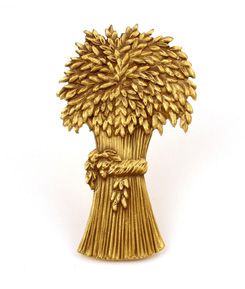
\includegraphics[scale=0.5]{photos/sheaf}}
  \put(-1.5,-29){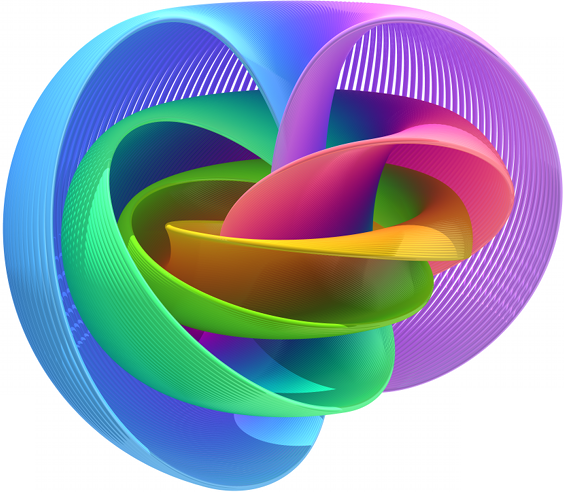
\includegraphics[scale=0.15]{photos/hopf-fibration}}
\end{picture}
\vspace{-2em}

\begin{center}
  \huge
  Dienstag, 20. Januar 2015, 10:00 Uhr, 1008/L1 \\[0.5em]
  Meru Alagalingam, Ingo Blechschmidt: \\
  \textbf{A gentle introduction to the Leray spectral sequence}
  \vfill
  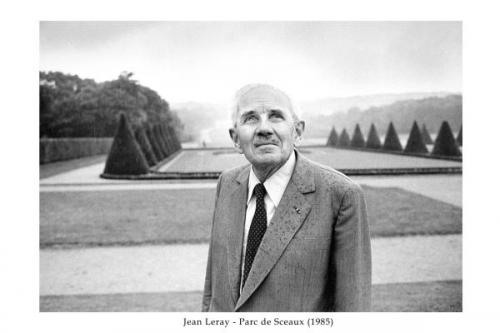
\includegraphics[scale=0.9]{photos/leray}
  \vfill

  \Large
  \begin{minipage}{0.89\textwidth}
    \setlength\parskip{\medskipamount}
    \vspace{0.3em}
    ``In the late 1940s and early 1950s all of us were studying Leray’s papers to
    try to understand how he got the marvelous results he claimed. To be perfectly
    frank, I never got to first base in this enterprise, it was very frustrating.
    Leray was a horrible expositor.'' -- Bill Massey

    The results Massey refers to are the numerous applications of the Leray
    spectral sequence, which Leray invented in the 1940s. This is an algebraic tool
    which, given any continuous map $f : X \to Y$ (not necessarily a bundle or
    fibration), relates the cohomology of the base space~$Y$, the total space~$X$,
    and the fibers of~$f$. To this end, Leray had to introduce sheaves and sheaf
    cohomology.

    The talk will give an introduction to the Leray spectral sequence, setting up
    only those concepts of sheaf theory and homological algebra which are strictly
    needed for the task. Many examples will illustrate its use. Along the way, we
    will also understand the conceptual background of the Mayer--Vietoris sequence
    and its generalization to coverings consisting of more than two sets.

    Basic familiarity with algebraic topology is required, but no prior exposure to
    sheaves and spectral sequences is assumed. After the talk, you will have the
    working knowledge to apply the Leray spectral sequence in your studies.
  \end{minipage}

  \vfill
  \small
  Arbeitsseminar Geometrie/Topologie \\
  Sven Prüfer, Christopher Wulff
\end{center}

\end{document}
